\section{DTE}
\label{sec:dte}
Die DTE\footnote{\emph{DTE} lässt sich mit \emph{Verteilungsumwandelnde Codiermaschine} übersetzen, weshalb in dieser Ausarbeitung der feminine Genus für den Fachbegriff verwendet wird.}, Abkürzung für \emph{distribution-transforming encoder}, dient zum Abbilden einer Nachricht $M$ aus dem Message Space $\mathcal{M}$ auf einen Seed $S$ aus dem Seed Space $\mathcal{S}$. Gleichermaßen soll sie die Möglichkeit bieten, von einem Seed auf die ursprüngliche Nachricht abzubilden. Eine DTE ist also ein Tupel von Algorithmen
$$DTE = (encode, decode)$$
wobei $encode$ einen meist randomisierten Algorithmus der Form $\mathcal{M} \rightarrow \mathcal{S}$ und $decode$ einen deterministischen Algorithmus der Form $\mathcal{S} \rightarrow \mathcal{M}$ beschreibt.

Ein DTE-Schema $(encode, decode)$ wird als \emph{korrekt} bezeichnet, wenn für jede Nachricht $M \in \mathcal{M}$, die mit $encode$ in den Seed Space $\mathcal{S}$ und mit $decode$ anschließend wieder in den Message Space $\mathcal{M}$ abgebildet wird, das Resultat wieder die ursprüngliche Nachricht $M$  ist. Formal kann dies geschrieben werden als
$$P(decode(encode(M)) = M) = 1 \qquad \forall M \in \mathcal{M}$$
wobei P ein Maß für die Wahrscheinlichkeit für das in den Klammern stehende Ereignis ist.

Bei der Konstruktion einer DTE ist die Korrektheit nicht das einzige Kriterium, welches es zu beachten gilt. Wichtig ist ebenfalls, die Verteilung der Wahrscheinlichkeiten der Nachrichten im Message Space zu kennen. Sie wird mit $p_m$ bezeichnet. Entsprechend dieser Wahrscheinlichkeiten wird einer Nachricht eine Anzahl von Seeds zur Kodierung zugewiesen. Je wahrscheinlicher eine Nachricht ist, desto mehr Seeds werden ihr zugewiesen.

Bei der Verschlüsselung einer Nachricht $M \in \mathcal{M}$ weist der Algorithmus $encode$ dieser Nachricht einen Seed entsprechend ihrer Wahrscheinlichkeit zu. Da es jedoch mehr als einen Seed zu einer Nachricht geben kann, handelt es sich bei $encode$ um einen randomisierten Algorithmus, der zufällig und gleichverteilt einen der möglichen Seeds auswählt. Da diese Kodierungs-Methode nicht deterministisch ist, handelt es sich bei $encode$ um keine Funktion oder Abbildung im mathematischen Sinne. Der Begriff \emph{Abbildung} ist dennoch eine passende Umschreibung für das Vorgehen zur Kodierung der Nachricht, mit einem Seed als Resultat.

Jede Nachricht kann also durch mehr als einen Seed dargestellt werden, aber jeder Seed verweist auf genau eine Nachricht (zu sehen in Abbildung \ref{fig:dte}).

\begin{figure}[!h]
\center
\begin{tikzpicture}
	% Linke Seite
	\draw (1,2) rectangle (4, 12);
	\draw (1,4) -- (4, 4);
	\draw (1,6) -- (4, 6);
	\draw (1,8) -- (4, 8);
	\draw (1,10) -- (4, 10);
	% Rechte Seite
	\draw (7,4) rectangle (10, 12);
	\draw (7,6) -- (10, 6);
	\draw (7,8) -- (10, 8);
	\draw (7,10) -- (10, 10);
	% Verbindungen
	\draw (4,11) -- (7, 11);
	\draw (4,9) -- (7, 11);
	\draw (4,7) -- (7, 9);
	\draw (4,3) -- (7, 5);
	% Labels links
	\node at (2.5, 11) {$S_{1}$};
	\node at (2.5, 9) {$S_{2}$};
	\node at (2.5, 7) {$S_{3}$};
	\node at (2.5, 5) {$\dots$};
	\node at (2.5, 3) {$S_{|\mathcal{S}|}$};
	% Labels rechts
	\node at (8.5, 11) {$M_{1}$};
	\node at (8.5, 9) {$M_{2}$};
	\node at (8.5, 7) {$\dots$};
	\node at (8.5, 5) {$M_{|\mathcal{M}|}$};
	% Labels unten
	\node at (8.5, 1) {$\mathcal{M}$};
	\node at (2.5, 1) {$\mathcal{S}$};
	% Pfeile
	\draw [<-] (4,1.2) -- node [above] {$encode(M)$} ++ (3,0) ;
	\draw [->] (4,0.8) -- node [below] {$decode(S)$} ++ (3,0);
\end{tikzpicture}
\caption{Relationen zwischen $\mathcal{M}$ und $\mathcal{S}$}
\label{fig:dte}
\end{figure}

Somit ist leicht zu erkennen, dass es sich bei $decode$ um einen deterministischen Algorithmus handelt. Der Begriff \emph{Abbildung} wäre in diesem Fall auch mathematisch korrekt.

Wie schon beschrieben, sollte die Wahrscheinlichkeitsverteilung der Nachrichten so gut wie möglich durch die DTE nachgeahmt werden. Juels und Ristenpart \cite{EURO2014} führen hierfür eine neue Verteilung $p_d$ ein --- die Verteilung, die die DTE über den Message Space $\mathcal{M}$ erzeugt. Diese wird definiert als die Wahrscheinlichkeit, dass zufällig und gleichverteilt gewählte Seeds durch die $decode$-Funktion auf eine bestimmte Nachricht $M$ abgebildet wird.

$$p_d(M) = P(M' = M : S \overset{<r>}{=} \mathcal{S} ; M' = decode(S))$$

Eine intuitivere Definition von $p_d$ wäre

$$p_d(M) = \frac{|\mathcal{S}_M|}{|\mathcal{S}|}$$

Dabei sei $\mathcal{S}_M$ die Menge aller Seeds, die durch den $decode$-Algorithmus wieder auf $M$ abgebildet werden. Diese Definition bezieht sich auf die diskrete Gleichverteilung des Seed Spaces und die dadurch anwendbare Laplace-Formel.

Bei der Erstellung einer DTE sollte darauf geachtet werden, dass $p_d \approx p_m$ gilt. Bei einer perfekten DTE würde eine Gleichheit der Verteilungen gelten.

\subsection{Generierung einer DTE mithilfe der Inversionsmethode}

Ein mögliches Vorgehen zur Erstellung einer DTE, die von Juels und Ristenpart in \cite{EURO2014} vorgeschlagen wird, ist die Nutzung der sogenannten Inverse Sampling Methode, zu Deutsch Inversionsmethode. Sie wird in der Informatik und Stochastik angewendet, ``um aus gleichverteilten Zufallszahlen andere Wahrscheinlichkeitsverteilungen zu erzeugen.'' \cite{WIKIInv} Meist wird dieses Verfahren in der Informatik für die Simulation von Zufallsvariablen, wie beispielsweise dem Monte-Carlo-Verfahren, verwendet. Dabei wird einer Rechteckverteilung $R(0,1)$ eine neue Wahrscheinlichkeitsverteilung zugewiesen. So kann ein Computer Zufallszahlen erzeugen, die in einer beliebigen, neuen Verteilung liegen, im Gegensatz zu den normalerweise von ihm generierbaren Zahlen im Intervall $[0,1)$.

Wie schon beschrieben wurde, muss für die Generierung einer DTE $p_m$, also die Wahrscheinlichkeitsverteilung für die Nachrichten des Message Spaces, bekannt sein. Nach den Regeln der Stochastik hat jede Nachricht eine Wahrscheinlichkeit im Intervall $(0,1)$, wobei die Summe aller Wahrscheinlichkeiten gleich $1$ sein muss. Es sei hier explizit darauf hingewiesen, dass die Intervallränder $0$ und $1$ als Wahrscheinlichkeiten für Nachrichten ungeeignet sind. Gilt nämlich für eine Nachricht $M \in \mathcal{M}$ $P(M) = 0$, dann ist das Vorkommen dieser Nachricht nicht möglich und sollte somit gar nicht beachtet werden. Ein Vorkommen im Message Space ist damit überflüssig. Gilt andererseits für $M$ $P(M) = 1$, so ist dies die einzig mögliche Nachricht. Dann ist es nicht sinnvoll, Honey Encryption zu verwenden, da ein potentieller Angreifer zum eindeutigen Entschlüsseln nicht einmal den Ciphertext kennen müsste. Der Angriff wäre trivial.

Eine DTE wird mit diesem Vorwissen nun wie folgt erstellt: Es wird die Verteilungsfunktion $F_m$ der Verteilung $p_m$ genutzt. Gegeben sei dafür eine Ordnung der Nachrichten im Message Space $\mathcal{M} = \{M_1, \dots, M_{|\mathcal{M}|}\}$. Die Verteilungsfunktion einer Nachricht $F_m(M_i)$ ist nun die Summe der Wahrscheinlichkeiten der ersten $i$ Nachrichten.

$$F_m(M_i) = \sum_{k = 1}^{i} P(M_k)$$

Um die Grenzen festzulegen, sei $F_m(M_0) = 0$ und logischerweise $F_m(M_{|\mathcal{M}|}) = 1$. Die Visualisierung für eine Verteilungsfunktion solcher Art --- hier des Beispiels aus Abschnitt \ref{sec:funktionsweise-beispiel} --- ist in Abbildung \ref{fig:Verteilungsfunktion} zu sehen.

\begin{figure}[!h]
\center
\begin{tikzpicture}
% Achsen:
	% x-Achse
	\draw [->] (-1,0) -- (5,0) node [right] {$i$};
	\draw (1,-0.1) -- (1,0.1);
	\draw (2,-0.1) -- (2,0.1);
	\draw (3,-0.1) -- (3,0.1);
	\draw (4,-0.1) -- (4,0.1);
	\node at (0.5, -0.5) {$0$};
	\node at (1.5, -0.5) {$1$};
	\node at (2.5, -0.5) {$2$};
	\node at (3.5, -0.5) {$3$};
	% y-Achse
	\draw [->] (0,-0.5) -- (0,2.5) node [above] {$F_m(M_i)$};
	\draw (-0.1,0.5) --++ (0.2,0);
	\draw (-0.1,1) --++ (0.2,0) node [left] {$0.5\ \ $};
	\draw (-0.1,1.5) --++ (0.2,0);
	\draw (-0.1,2) --++ (0.2,0) node [left] {$1\ \ $};
	% Linien
	\draw [thick] (-1,0) -- (1,0);
	\draw [thick, |-] (1,0.5) -- (2,0.5);
	\draw [thick, |-] (2,1) -- (3,1);
	\draw [thick, |-] (3,2) -- (5,2);
\end{tikzpicture}
\caption{Die Verteilungsfunktion $F_m$ mit $M_1 = r$, $M_2 = g$ und $M_3 = b$}
\label{fig:Verteilungsfunktion}
\end{figure}

Sei nun der Wertebereich aller Seeds $S \in \mathcal{S}$ das Intervall $[0,1)$. Ein Seed $S$ wird dann in seine Ursprungsnachricht zurückgeführt (\emph{decode}-Algorithmus), indem die Nachricht $M_i$ gefunden wird, für die $F_m(M_{i-1}) \leq S < F_m(M_i)$ gilt. Wenn als Beispiel der Seed zwischen der Summe der ersten 5 und 6 Nachrichtenwahrscheinlichkeiten liegt, dann gibt der \emph{decode}-Algorithmus $M_6$ als ursprüngliche Nachricht zurück. Eine anders geschriebene und leichter in Programmen umsetzbare Schreibweise der Übersetzung von Seed in Nachricht ist

$$min_i\{F_m(M_i) > S\}$$

Anschaulich sei ein Maßband der Länge 1 betrachtet, auf der die Nachrichten entsprechend ihrer Wahrscheinlichkeiten aufeinanderfolgend und disjunkt aufgetragen (in Abbildung \ref{fig:decode} wieder am Beispiel aus Abschnitt \ref{sec:funktionsweise-beispiel} zu sehen) wurden. Ein Seed liegt nun irgendwo auf der Länge des Maßbandes. An dieser Stelle liegt auch eine Nachricht $M_i$, die dann als ursprüngliche Nachricht ausgegeben wird. Liegt der Seed dabei auf der Grenze zweier Nachrichten, wird die weiter rechts liegende zurückgeliefert.

Beispielsweise wird $decode$ mit dem Parameter $0.4$ aufgerufen. Auf dem Maßband liegt an dieser Stelle $M_2$, weshalb diese als ursprüngliche Nachricht zurück gegeben wird.

\begin{figure}[!h]
\center
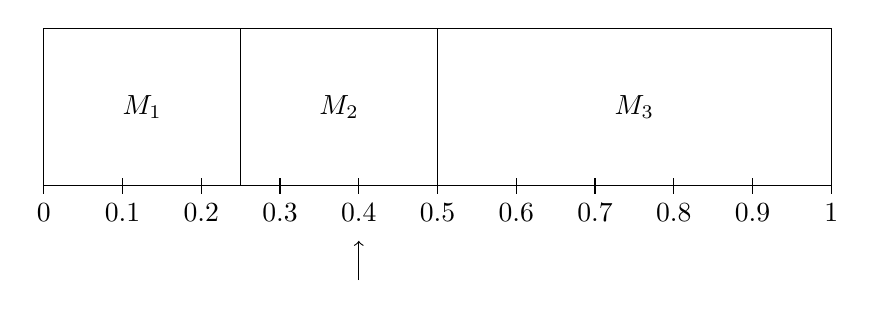
\begin{tikzpicture}
	% Kaesten
	\draw (0,0) rectangle (2.5,2) node [midway] {$M_1$};
	\draw (2.5,0) rectangle (5,2) node [midway] {$M_2$};
	\draw (5,0) rectangle (10,2) node [midway] {$M_3$};
	% Skala
	\foreach \x [evaluate=\x as \result using \x*0.1] in {0, 1, ..., 10} {
		\draw (\x, -0.1) -- (\x, 0.1) node [below=0.2cm] {\pgfmathprintnumber{\result}};
	}
	% Pfeil
	\draw [->] (4, -1.2) -- (4, -0.7);
\end{tikzpicture}
\caption{Ein Maßband als Analogie zum \emph{decode}-Algorithmus}
\label{fig:decode}
\end{figure}

Es ist an der anschaulichen Darstellung unschwer zu erkennen, dass die Verteilung $p_m$ in der DTE wieder zu finden ist. Die Wahrscheinlichkeit einer Nachricht wird durch ihre Breite dargestellt. Da die Seeds gleichverteilt sind, ist es leichter, einen besonders breiten Abschnitt zu treffen, als einen schmaleren.

Bisher wurde der \emph{decode}-Algorithmus betrachtet. Der \emph{encode}-Algorithmus ist ähnlich anschaulich zu erklären. Dieses Mal wird eine Nachricht gewählt, die auf dem Maßband liegt. Der Bereich an Werten auf dem Maßband, der von dieser Nachricht abgedeckt wird, wird als Grundlage für eine Auswahl eines Seeds verwendet. Dabei wird zufällig gleichverteilt ein Wert aus diesem Bereich ausgewählt.

Auf die Verteilungsfunktion bezogen ist ein Seed, der aus der Nachricht $M_i$ generiert wird, eine reelle Zahl im Intervall $[F_m(M_{i-1}), F_m(M_i))$. Die Auswahl aus diesem Intervall lässt sich mithilfe eines Computers recht einfach bewerkstelligen, da dieser im Normalfall reelle Zufallszahlen im Intervall $[0,1)$ generieren kann --- Sicherheitsaspekte und -bedenken bezüglich vom Computer generierter Zufallszahlen seien in dieser Ausarbeitung vernachlässigt.

Auch hier ist klar, dass es ein größeres Seedintervall für eine Nachricht gibt, je wahrscheinlicher diese Nachricht ist. Daher ist diese Eigenschaft einer guten DTE ebenfalls gegeben.

Um die erzeugte DTE praktisch anwenden zu können, muss noch das Problem der Übersetzung der stetigen Werte zwischen $[0,1)$ in die diskreten Werte von in Binärzahlen angegebenen Seeds des Seed Spaces, welcher tatsächlich verwendet wird. Die Anzahl der Seeds sollte so gewählt werden, dass die Abweichungen der relativen Seed-Bereiche einer Nachricht in beiden Repräsentationen möglichst klein sind. Je größer die Abweichungen nämlich sind, desto mehr verzerrt sich die Verteilung der DTE. Die erstrebenswerten Eigenschaften einer guten DTE wären damit nicht mehr gegeben und es könnte zu einem Sicherheitseinbruch der Honey Encryption mit dieser DTE kommen.

\subsection{Eine DTE für private RSA-Schlüssel}
\label{sec:dte-rsa}

Das folgende Beispiel ist entnommen aus \cite{EURO2014}.

Bei RSA handelt es sich um einen asymmetrischen Verschlüsselungsalgorithmus, d.h. das Verfahren beruht auf einem öffentlichen und einem privaten Schlüssel. Zur Generierung der Schlüssel (heutiger Stand: 2000 Bit, siehe \cite{BSI2014}) wählt man zwei große  Primzahlen \(p\) und \(q\) und errechnet aus ihnen öffentlichen und privaten Schlüssel (zu Details siehe \cite{Schneier2006}). RSA wird beispielsweise bei SSL/TLS oder SSH eingesetzt. Für die Anwendung von Honey Encryption ist jedoch nur der zweite Fall geeignet, denn bei SSL/TLS ist der öffentliche Schlüssel des Servers bekannt und so ließe sich leicht nachprüfen, ob der richtige private Schlüssel entschlüsselt wurde. 

Bei SSH lässt sich Honey Encryption jedoch anwenden. In diesem Fall wird der öffentliche Schlüssel zum Zweck der Authentifizierung auf dem Server gespeichert, den man erreichen möchte (und steht somit dem Angreifer nicht zur Verfügung). Der private Schlüssel (genauer \(p\) und \(q\) zusammen mit weiteren berechneten Werten, um die Ver- bzw. Entschlüsselung nach dem Chinesischen Restsatz zu erleichtern) wird verschlüsselt auf dem Clientsystem gespeichert.

Zur Erstellung einer DTE für RSA-Schlüssel muss betrachtet werden, wie die Primzahlen \(p\) und \(q\) (im Folgenden werden Primzahlen aus dem Intervall \([2^{l-1},2^l)\) gefordert) erhalten werden. Normalerweise werden zufällige Zahlen aus dem Intervall gewählt und durch einen Primzahltest (z.B. Miller-Rabin-Test) auf Primzahleigenschaften hin überprüft. Dies wird solange wiederholt, bis man zwei Primzahlen gefunden hat. 

% Guck nochmal nach, wieso l-2
Ein naiver Ansatz für eine DTE wäre es, die beiden gefundenen Primzahlen als \((l-2)\)-Bitstrings zu dekodieren (die auf jeden Fall vorhandene führende 1 ist implizit und wird ausgelassen). Da jedoch bei der Entschlüsselung dann auch Nicht-Primzahlen entstehen würden (und zwar nach dem Primzahlsatz mit etwa Wahrscheinlichkeit \(1-\frac{1}{l}\)), würde ein Angreifer viele Ausgaben von vornherein als nicht plausibel erkennen können.

Daher schlagen die Autoren in \cite{EURO2014} ein anderes Vorgehen vor. Zur Kodierung von \(p\) und \(q\) wird ein Vektor von \(t\) zufälligen \((l-2)\)-Bitstrings angelegt. Per Primzahltest werden die Zahlen überprüft. Die ersten beiden Primzahlen in dem Vektor werden durch \(p\) und \(q\) ersetzt. Enthält der Vektor nur eine Primzahl, so wird diese durch \(p\) und die letzte Zahl durch \(q\) ersetzt. Enthält der Vektor keine Primzahlen, so ersetzen \(p\) und \(q\) die letzten beiden Zahlen. Beim Dekodieren werden die ersten beiden Primzahlen im Vektor ausgegeben. Wenn der Vektor keine zwei Primzahlen enthält, so werden fest kodierte Primzahlen ausgegeben.

Es lässt sich zeigen, dass ein Angreifer, der versucht \(p\) und \(q\) per Brute-Force-Angriff zu erhalten, eine Erfolgswahrscheinlichkeit von höchstens \((1-\frac{2}{3l})^{t-1}\) besitzt (ebenfalls \cite{EURO2014}). Damit lässt sich diese Wahrscheinlichkeit also durch Nutzung eines größeren Vektors verringern (allerdings auf Kosten größeres Speicherplatzbedarfs).

Ein anderer Ansatz, der in \cite{EURO2014} erwähnt wird, ist die Kodierung des Seeds/Keys, der zur Initialisierung des Zufallszahlengenerators verwendet wurde, um \(p\) und \(q\) zu generieren. Eine DTE wäre trivial, da es sich bei dem Seed/Key im Allgemeinen um einen kurzen, zufällig gleichverteilten Bitstring handelt.
